\scanpage{7}
$C_1$ peut aussi se mettre sous la forme

$7^\circ)$ Pour $\forall\ S'\longrightarrow S$ [avec $S'$ \deleted{local} noeth. \inserted{[local]} complet [irréduct. de dim $1$] et $S'_0$ sous-\deleted{\unsure{pré}}schéma défini par un idéal nilpotent [de carré nul], \deleted{toute} ouvert $U\subset S'$ \inserted{d'adhérence schématique $S'$} [$U=S'-\text{pt fermé}$], et \deleted{section de $F_T$} $S'$-morphisme $\unsure{\eta|y}_0:S'_0\mathrel{\unsure{-|\longrightarrow}}F_{S'}$, \deleted{\unsure{tel que et}} \deleted{$\unsure{\eta|y}:S'$} si $\unsure{\eta|y}_0|U_0$ se prolonge en $\unsure{\eta|y}_{\unsure{U}}:U\mathrel{\unsure{-|\longrightarrow}}F_{S'}$, alors $\unsure{\eta|y}_0$ se prolonge en $\unsure{\eta|y}:S'\mathrel{\unsure{-|\longrightarrow}}F_{S'}$.
\margin{\figure{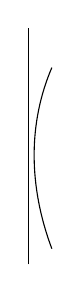
\begin{tikzpicture}\draw (0,0)--(0,3);\draw (.3,.2)..controls (0,1) and (0,1.8)..(.3,2.5);\end{tikzpicture}}}

[\uline{NB} Cette condition est \uline{vide} si $F\longrightarrow S$ est étale]

\margin{Cela se met sous la forme :}
\margin{\deleted{\illegible{1}}}
$8^\circ)$ Soit $S'$ sur $S$ noeth irréductible, \inserted{de pt gén. $x$} $S'_0$ défini par un idéal \deleted{nilpotent}, $\unsure{\eta|y}:S'_0\longrightarrow F_{S'}$, supposons que $\unsure{\eta|y}$ soit modulaire \inserted{(i.e. étale)} en $x$, alors il est modulaire au voisinage de $x$.

\figure{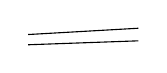
\begin{tikzpicture}\draw (0,0)--(1.4,.08);\draw (0,-.13)--(1.4,-.08);\end{tikzpicture}}

Revenons au cas général, \inserted{(pas néc. non ram.)} je dis que (A) et (B) peuvent se remplacer par

\margin{(D)}
$(D_1)$ Si $S'$ noeth sur $S$, $\unsure{X|Z}$ \deleted{\unsure{qu. fini}} sur $S'$, et $\unsure{\eta|y}:\unsure{X|Z}\longrightarrow F_{S'}$ un $S'$-morphisme, l'ens des pts où $\unsure{\eta|y}$ est inf\textsuperscript{t} étale est \uline{ouvert} ; \deleted{Et}
\margin{\figure{\begin{tikzpicture}\draw (0,0)--(0,1.6);\end{tikzpicture}}}
\deleted{[Conditions analogues pour}
\diagram{\begin{tikzcd}\deleted{F}\arrow[r,"\deleted{\mathrm{diag}}"]&\deleted{F\times_S F}\end{tikzcd}}
\deleted{, puis $\forall$ \unsure{changement} de base, \unsure{pour} $\unsure{\eta|y}$ \unsure{capturant} \unsure{l'expression} \unsure{des} $7^\circ$ et $8^\circ$]}
\deleted{\unsure{et} \unsure{sur} \uline{\unsure{un}} voisinage)}
\deleted{il en est de même \unsure{pour} le \unsure{foncteur} $X\times_{F_{S'}}X$ sur $S'$, \unsure{pour} \unsure{le} \unsure{morphisme}}
\diagram{\begin{tikzcd}\deleted{\unsure{X\times_{S'}X|X_{S'}}}\arrow[r]&\deleted{\unsure{S'}}\end{tikzcd}}
\deleted{\unsure{pour} $\unsure{T}$ \unsure{plongé} dans $X\times_S X$, de sorte que \unsure{cette} condition s'exprime au moyen de $7^\circ$ et $8^\circ$].}
\mspage{6}
